\documentclass[review]{elsarticle}

\usepackage{lineno,hyperref}
\usepackage[czech]{babel}
\usepackage[utf8]{inputenc}   % pro unicode UTF-8
\modulolinenumbers[5]

\journal{Journal of EAAI}

%%%%%%%%%%%%%%%%%%%%%%%
%% Elsevier bibliography styles
%%%%%%%%%%%%%%%%%%%%%%%
%% To change the style, put a % in front of the second line of the current style and
%% remove the % from the second line of the style you would like to use.
%%%%%%%%%%%%%%%%%%%%%%%

%% Numbered
%\bibliographystyle{model1-num-names}

%% Numbered without titles
%\bibliographystyle{model1a-num-names}

%% Harvard
%\bibliographystyle{model2-names.bst}\biboptions{authoryear}

%% Vancouver numbered
%\usepackage{numcompress}\bibliographystyle{model3-num-names}

%% Vancouver name/year
%\usepackage{numcompress}\bibliographystyle{model4-names}\biboptions{authoryear}

%% APA style
%\bibliographystyle{model5-names}\biboptions{authoryear}

%% AMA style
%\usepackage{numcompress}\bibliographystyle{model6-num-names}

%% `Elsevier LaTeX' style
\bibliographystyle{elsarticle-num}
%%%%%%%%%%%%%%%%%%%%%%%

\begin{document}

\begin{frontmatter}

%\title{Elsevier \LaTeX\ template\tnoteref{mytitlenote}}
%\tnotetext[mytitlenote]{Fully documented templates are available in the elsarticle package on \href{http://www.ctan.org/tex-archive/macros/latex/contrib/elsarticle}{CTAN}.}
\title{Evolution of Digital Code}

%% Group authors per affiliation:
\author{Kateřina Káňová}%\fnref{myfootnote}}
\address{}
%\fntext[myfootnote]{Since 1880.}

%% or include affiliations in footnotes:
%\author[mymainaddress,mysecondaryaddress]{Elsevier Inc}
%\ead[url]{www.elsevier.com}

%\author[mysecondaryaddress]{Global Customer Service\corref{mycorrespondingauthor}}
%\cortext[mycorrespondingauthor]{Corresponding author}
%\ead{support@elsevier.com}

%\address[mymainaddress]{1600 John F Kennedy Boulevard, Philadelphia}
%\address[mysecondaryaddress]{360 Park Avenue South, New York}

\begin{abstract}
In this participation we discuss the possibility of connecting computer evolution and self-replicating structures. The structures are similar to computer viruses but they differ substantially in several aspects of behaviour. At the beginning of this paper the familiarization with the issue of computer viruses and evolution techniques takes place. 

Self-replicating structures were inspired by computer viruses so they are quite similar to them. On the other hand, they are different in both structure and behaviour. The first part refers to computer viruses themselves and describe their structure and behaviour.

Special attention is paid to the SOMA algorithm because this technique was used for experiments. SOMA algorithm is evolutionary technique that uses swarm intelligence to find the best solution of the given problem.

The question is, if there are any computer viruses that could evolve in computer environment. If so, that means that other computer programs (not only viruses) should be able to evolve too. This paper shows that computer program can be evolved in order to get better solution for given problem and therefore we can believe that there are some computer viruses using evolution too. This shows us new security problem that we should face in the future. 

At the end, there are some experiments which show how evolution of code was going and there is summary of gotten results.

\end{abstract}

\begin{keyword}
%\texttt{elsarticle.cls}\sep \LaTeX\sep Elsevier \sep template
%\MSC[2010] 00-01\sep  99-00
evolutionary algorithms
\end{keyword}

\end{frontmatter}

%\linenumbers

\section{Introduction}
Due to still emerging technologies and due to modernization and digitalization of almost all processes, more and more information about us and about our lives are stored in digital form. Talking about numbers of our credit cards, medical records or information about our current position, all of these data are saved on servers and therefore there is a possibility of a hacking attack and stealing data. 

Computer systems are getting more and more sophisticated so viruses, which attack these systems, have to get more sophisticated too. On the other hand, some of the systems are insufficiently secured despite warnings of public about privacy and about posting their data on internet. These systems are an easy target of an attack.

The fact, that a hacker finds a flaw in a system, that can be abused, doesn't have to be a bad news. There are "white hackers" as well, hackers who help securing systems. They report flaws they find so they can be fixed. Unfortunately, some companies don't care about these warnings and don't fix the flaws in their systems. But situation is getting better - some companies pays for white hackers and try to make their system as secure as possible. 

To protect your own computer, you can obviously use some antivirus protection. There is a great number of companies that specialize on the issue. To protect your computer and to destroy a virus, an antivirus program have to find the virus first. This is probably the greatest challenge, because there are many modifications of each individual virus. There are also viruses that can change their body by themselves, so they make antivirus job more difficult.

Is it possible for a code structure to evolve, to change itself to be better than its older variant? Computer viruses are one of the best structures to test this idea. Hence the self-replication structure (SS) is defined as a virus. \textbf{SS isn't a real virus -- it does not pose any threat, it's only there to test files that are created only for testing purposes. Users can set testing files and HDD partitions for the attack and so this "virus" is strictly controlled. At the end of the program execution, all infected files are removed from all partitions.}

Information below is divided into three main parts. The first one aims to provide theoretical information that serves as a basis for this work. In the second part you can read about implementation of the program. The results of the work are summarized in the last part.


\subsection{Computer viruses and their sibblings}
To understand the behaviour SS, it is important to understand computer viruses themselves. Although the word "virus" is widely used, it is hard to tell its current meaning. Some use word "virus" for a group of harmful codes, but virus is just specific type of computer malware. If we talk about malware, we mean harmful code that works to an attacker's advantage. Its specific functions allow us to classify it in many ways. One of the classification groups are viruses.
\vspace{5pt}

The computer viruses and biological ones has a lot of similarities. \cite{viryHak} \cite{webroot} It is a cell of information that is able to find a host and to spread. \cite{norton} Although there are some similarities between a computer virus and a biological one, there are some distinctions too. The following Table \ref{diverg} is an overview of the diverging attributes.


\begin{table}[!h]
	\centering
	\caption{Divergence of computer and biological viruses}
	\label{diverg}
	\small
\begin{tabular}{ p{6cm} | p{6cm} }
%	\toprule
	Biological virus & Computer virus \\
%	\midrule
	They can't self-replicate. They need infected cells. & To reproduce they need infected files. \\
	They attack specific cells. & They attack specific files. \\
	They change the infected cell's DNA to replicate. & They change the infected file's data to replicate. \\
	They take control of part or of the whole cell. & They are executed before the original file. \\
	The cell is usually not infected twice by the same virus. & Most viruses don't infect the same file twice. \\
	Symptoms may not be exhibited or could be delayed. & Symptoms may not be exhibited or could be delayed. \\
	Viruses mutate. It is more difficult to find them and cure them. & They can mutate or include "safeguards". Finding and destroying them is more difficult. \\
	Cells can be vaccinated. & Files can be protected. \\
	\hline	
\end{tabular}
\end{table}


From the technical point of view we can define a virus as follows:
\vspace{5pt}

\textit{A virus can be described by a sequence of symbols which is able, when interpreted in a suitable environment (a machine), to modify other sequences of symbols in that environment by including a possibly evolved copy of itself.}
\vspace{5pt}

That means, that viruses don't spreed among computers over a network (as worms do) but they infect files in PCs. Because viruses need executoin of their program, they usually attack executable files. They can be searching for them on current disk or all disks in machine. So how can viruses be relocated from one PC to another? In fact there are many ways a virus can find your PC. \cite{webroot}

Some examples how virus can find your PC and spread through it are mentioned in the list below.

\begin{itemize}
	\item Sharing music, files or photos with other users.
	\item Visiting an infected website.
	\item Opening a spam e-mail or its attachment.
	\item Downloading free games, toolbars, media players and other system utilities.
	\item Installing mainstream applications without fully understanding their license agreements.
\end{itemize}

Although there are many antivirus programs on the market, they only deal with consequences of users' behaviour. Thus, if you are careful, you make work of your antivirus much easier. But there are more and more viruses and antivirus companies are still one step behind virus creators. So if you think twice about what you are doing on your PC (especially while connected to internet), you are the best antivirus protection that you can have. 

\subsubsection{Virus types}
Virus itself is a harmful piece of code often with a destructive payload . Even if it is not destructive, it is still harmful because it steals computing time and resources to do things you don't want your PC to do.
There are many virus types depending on the way they spread, the objects they infect, the way they infect these objects etc. \cite{panda}\\

\textbf{Differences in payload}\\
By a virus payload we mean its special - not common behaviour. Taken from \cite{definition}, page 46, it states:
\vspace{5pt}

\textit{'The existence of a payload -- in other words an offensive procedure -- is not an essential feature in characterizing a virus.'}
\vspace{5pt}

Some consider a virus behaviour (e.g. spreading, searching for files, infecting files) to be a part of its payload. Common use of the word 'payload' means an additional function with a special purpose -- it may send data to a hacker, watch a user's keyboard etc. The following section treats payload as a special functional part of a virus body.

\label{ref:payload}
Payload execution usually takes place by the end of virus lifecycle, after it has spread. Sometimes it is executed near the beginning, but there are some disadvantages to this approach. If such a virus gets discovered by e.g. an antivirus while performing its payload, it is usually terminated and thus has no chance to spread. That is why it is better to let viruses spread first and do some special activity later on. \cite{definition} Payload can be delayed and may wait for a special condition -- for example a specific date or a number of successful infections. \cite{definition}

We can simply divide virus payloads into lethal and non-lethal ones. \cite{definition} The lethal ones are those that corrupt files, steal data, corrupt or destroy systems or violate data integrity etc. Non-lethal ones are e.g. displaying some pictures or drawing a user's attention to such-and-such topic. \\

\textbf{Targets}\\
Viruses usually infect executable files (.EXE, .COM) and they abuse specific structures of these files. On the other hand, there are boot viruses that attack boot sectors or macros in documents created with Microsoft Office tools. Throughout the paper only viruses attacking .EXE files are studied -- for the purpose of creating SSs. Main focus is put on principles that are used by viruses attacking .EXE files. Other virus types are therefore not subject of further analysis.\\

\textbf{Ways of infection}\\
In general, viruses spread from file to file, that means they don't use network as worms do. They spread when the infected file with their code inside gets executed. There are, however, many ways in which files can be infected.
\vspace{5pt}

\begin{itemize}
\item \textbf{Rewriting}
\label{page:rewriting}

The rewriting virus is the simplest virus in terms of infection. It does not allow restoring of the infected files' content. The infected file is simply rewritten by the body of the virus while the body of the original program is lost. The figure \ref{pict:rewriting} shows the rewriting principle.

Using this method the resultant file can be either larger or smaller than the original one.

\begin{figure}[ht]
\center
\caption{Rewriting method of infection}
\label{pict:rewriting}
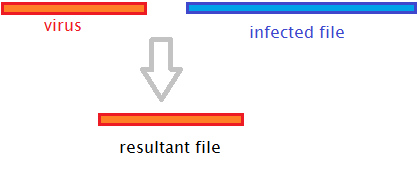
\includegraphics[scale=0.6]{pict/rewriting.png}
\end{figure}

\item \textbf{Prepending}
\label{page:prepend}
This method prepends virus code to the beginning of the infected program (so it gets executed before the original code) as you can see in the figure \ref{pict:prepend}. The original program is usually run from the virus body immediately after the virus is executed. Should it be run later, the user could suspect something and might start looking for the cause of the delay or he/she might scan the device with an antivirus.

Using this method the resultant file is always larger than the infected one.

The advantage is that the virus does not delete the content of the host file and it is fully restored so the user has no idea of the pending virus infection.

\begin{figure}[h!t]
\center
\caption{Prepending method of infection}
\label{pict:prepend}
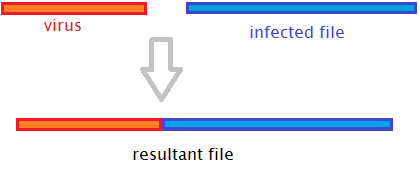
\includegraphics[scale=0.6]{pict/prepended.png}
\end{figure}

\item \textbf{Parasitical}
\label{page:parasitical}
The principle here is very similar to the one employed in the prepending method. The difference is that the original code isn't moved to the end, but split at the end of the virus body. The first part of the infected file is put to the end of the file. When the virus is run, it connects these parts together again and executes it in the way a prepending virus does. The figure \ref{pict:parasitical} explains how it works.

\begin{figure}[h!t]
\center
\caption{Parasitical method of infection}
\label{pict:parasitical}
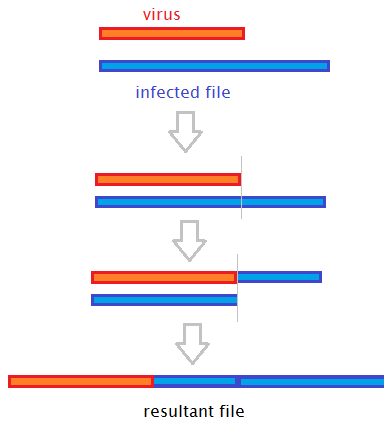
\includegraphics[scale=0.6]{pict/parasitical.png}
\end{figure}
\end{itemize}

\subsubsection{Other malware types}
Although virus is a cornerstone of SS, some other well-known types of malware are given here as well to realise difference between virus and other malwares.

\textbf{Trojan horse}

Trojan horse is malware similar to a virus with a single difference -- it cannot replicate. In a simple way we can say that trojan horse is the payload of a virus (Description of payload \ref{ref:payload}). Trojan horses are mostly executable files -- so they do not need a host file. To execute trojan horse code, the file containing a trojan horse only needs to be executed (by a user or by a process running on the device).
This is the reason why trojan horses try to look like useful or interesting applications -- to make users execute them. Hence the name.

Although a trojan horse cannot spread by itself, it is very often a part of a virus. This technique alows trojans to spread so you can encounter a trojan horse more often than you would expect. \cite{viryHak}

Basic types of trojan horses are summarized below.
\begin{itemize}
\item \textbf{Destructive trojan} is a type of trojan that has a destructive impact -- e.g. deleting files or formatting drives.

\item \textbf{Keyloggers} are programs that monitor pressed keys. They collect them and send them to the attacker. This type of infiltration can also be classified as spyware.

\item \textbf{Dropper} is like a giftbox hiding trojans in it. Droppers usually carry .EXE files. When executed, they let harmful programs spread in the device.

\item \textbf{Downloader} is a type of trojan horse similar to dropper, but it does not carry all of the harmful code with it. When downloader is executed, it simply downloads the needed content. Downloaders use predefined URLs to download content from. Great advantage is that if the content on the server is changed, the same downloader downloads the updated code and starts behaving differently.
\end{itemize}

\textbf{Backdoor}

\textit{Backdoor is a client-server application, whose abilities are very similar to commercial products such as pcAnyWhere, VNC or Remote Administrator.} \cite{viryHak}

The uniqueness of this type of malware is that it behaves in a way that a user cannot notice them. Controlling a device remotely may not mean anything bad, but if the activity is harmful, then we call the manipulating person a 'remote attacker'. \cite{viryHak} 

How does it work? The client side of the application is controlled by an attacker, while the server side is in a victim's device. Communication usually uses TCP/IP, which means that the attacker can be far away from the server side of the application. \cite{viryHak}

\textbf{Worm}

Worms are structures that work in a different way than viruses do. They don't infect files, rather they infect network packets themselves. That is why worms are not recognized by common antivirus programs. One of the most common impact of a worm infection is network congestion.

\textbf{Spyware}

Spyware is a type of malware that serves attackers as a spy. It collects information and send it back as in the case of backdoors. Unlike backdoors, spyware usually sends static data such as visited web pages or installed programs. The main reason why these programs exist is supposedly collecting data for targeted advertising.

\textbf{Adware}

Adware is something that makes you annoyed while working with your device. Adware should act as an advertisement on the web. Mostly the user agrees to installation of adware, but it can be a part of some product as well.

\textbf{Phishing}

Phishing attackers use web pages and forms and they persuade users to fill in their personal information. They achieve this by threatening users to make them do that. For example an attacker sends a message to a user that their account will be deleted or banned if they don't fill in the form. The problem is that these web pages and forms are very authentic so users have no idea they are being attacked.

\subsubsection{Where to find information on malware}
There are plenty of servers dealing with various topics on malware. Almost every antivirus company has its own website, own virus database and they present basic information about them. You can test files you have in your device at https://www.virustotal.com. Web pages of company symantec.com show some information too. 

Interesting summary is presented at http://www.avgthreatlabs.com/ww-en/virus-and-malware-information/ where you can find a map showing areas of virus detection. On the main page there are up to date information about the situation in the world for the past week. The figure \ref{pict:avg} shows information from the first week of April 2017.

\begin{figure}[!h]
\caption{Statistics taken from avgthreatlabs.com}
\label{pict:avg}
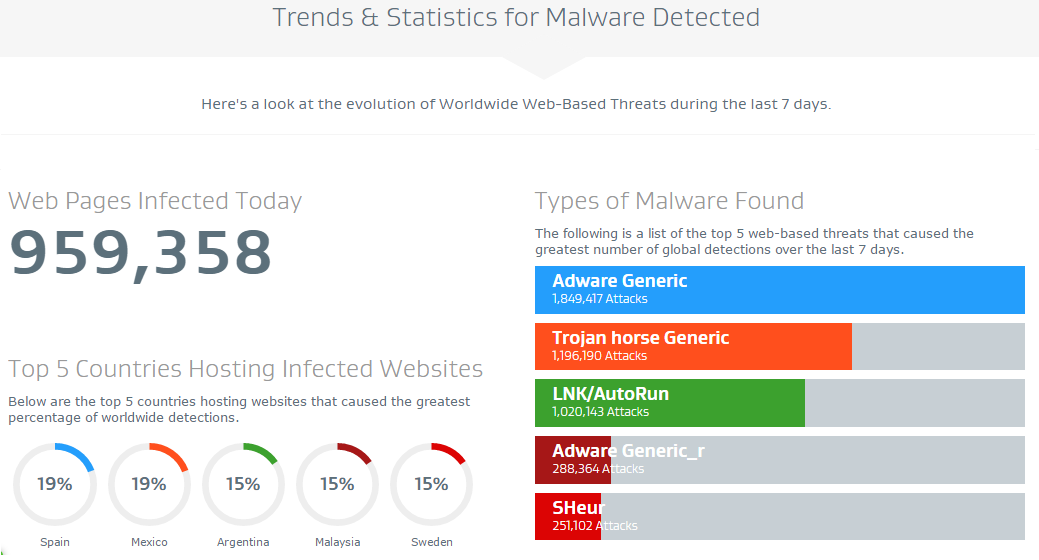
\includegraphics[scale=0.5]{pict/avgthreatlab.png}
\end{figure}

The ESET alows you to scan you PC online from https://www.eset.com/int/home/online-scanner/.

The company Symantec shows the number of malware which appeared depending on the malware type. For example email threads from last year \cite{symantec} are shown in the Fig. \ref{pict:email}.


\begin{figure}[!ht]
\centering
\caption{Statistics taken from symantec.com}
\label{pict:email}
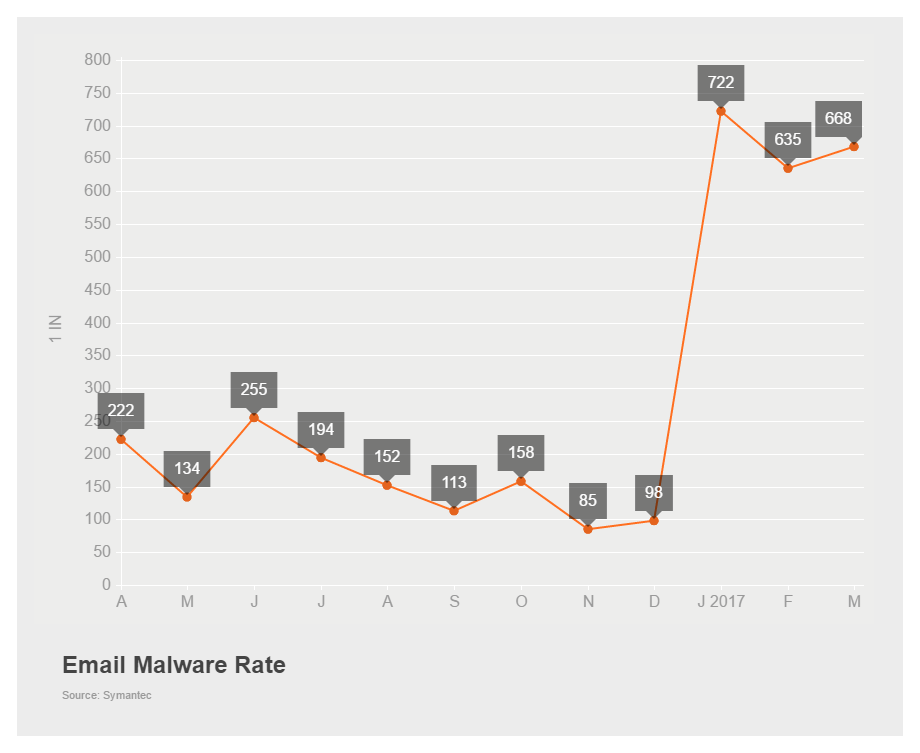
\includegraphics[scale=0.3]{pict/email.png}
\end{figure}


\newpage
\subsection{Evolution}
Evolution process is a term well-known from biology the definition of which sounds as follows: \\
\textit{'Evolution is the process by which the physical characteristics of types of creatures change over time, new types of creatures develop, and others disappear.'} \cite{evolution}
\vspace{5pt}

In the digital world, the first signs of evolution techniques can be dated to the early 1970s. At this time, genetic algorithms were discovered. A few years later the 'evolution strategies' were successfully used. \cite{zelinkaEvol}

Evolution is a simulation process that moves forward to find new (and better) solutions. The evolution of a digital structure is analogous to breeding a new biological species, e.g. a new dog breed. Entity is an instance of digital structure (or a particular dog). The best entities are crossbred to spread their genes. The goal is to get a new entity (new pupy) that should be better than its parents and closer to the desired features. The best offsprings become parents and the whole process repeats until we get a perfect entity. Unfortunately we don't usually get a \textit{perfect} entity in the real world. So we have to settle for the best solution after e.g. a limited number of evolution cycles or after a certain amount of time. 

The generalized view of evolutionary algorithm is shown in Fig. \ref{pict:soma}.

\begin{figure}[h!]
\caption{Evolutionary algorithm}
\label{pict:soma}
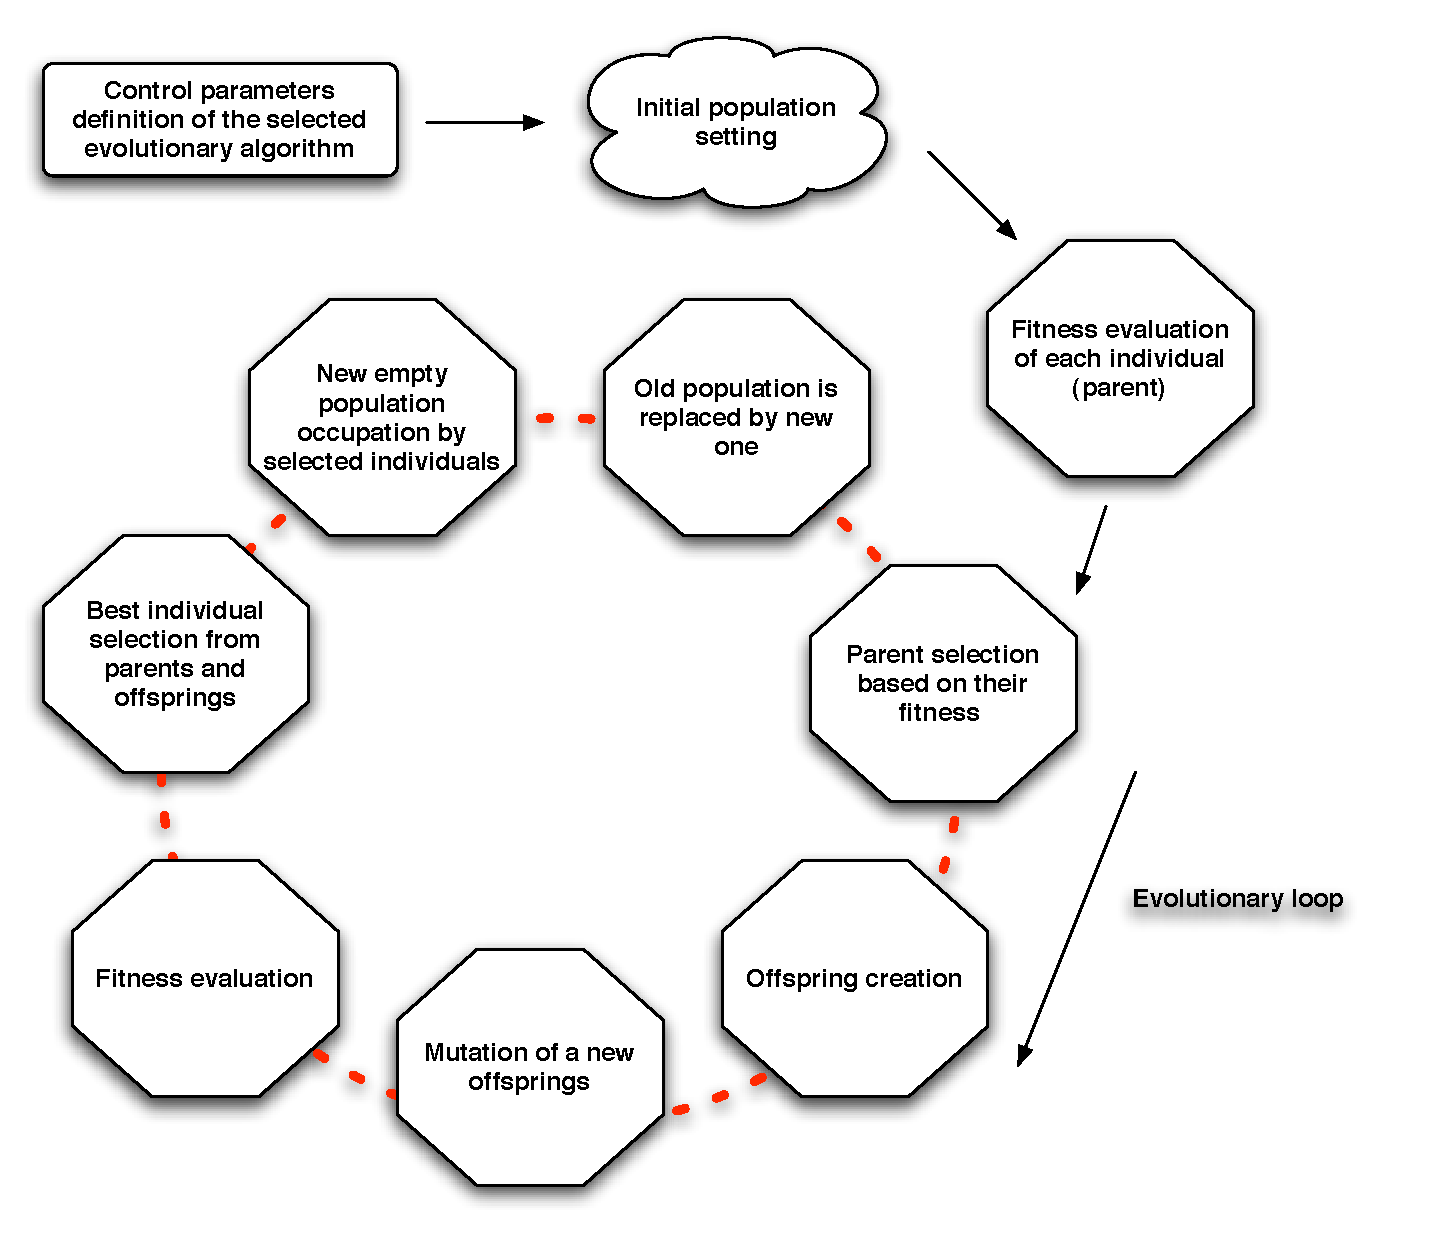
\includegraphics[scale=0.65]{pict/soma.pdf}
\end{figure}


Evolution in the digital are real world are very similar. The purpose of evolution is to get the best solution to a given problem. In the paper, evolution is applied in order to synthesize SSs with the best possible attributes.
\vspace{10pt}

\label{fitness} To compare two entities and to find out which one is better we need to establish a rating. This rating is called a \textbf{fitness} value and it is a result of \textbf{cost function}. \cite{soma} For example to evaluate which dog is better we should consider its height, color, behaviour, hair length and so on. If we want to breed a new computer virus, such a rating would make no sense. That means the cost funtion (rating system) depends on the problem we are trying to solve. If we talk about a virus, we want to have a rating that depends on the length of code, the execution time etc.

As a general rule we can assume that the higher the fitness value the better the entity. The fitness value is normalized to be in the interval from zero to one.

In the thesis we want to obtain the best SS, which is composed of several parts. We seek an entity with the shortest code, the shortest time of execution and the smallest number of errors. And so in this case the lower the cost function value the better the entity.

\subsection{Principle of the SOMA algorithm}
To explain how SOMA works it is necessary to know basic terms from the evolution theory. A brief overview follows to refresh them. 
\vspace{10pt}

\noindent
\textbf{Entity} -- an entity used in the evolution process (we want to evolve SSs, so the entity here is one particular SS). \\
\textbf{Generation} -- a group of entities created in a single evolution cycle. \\
\textbf{Fitness value} -- the value that says us how "good" a particular entity is. \\
\textbf{Migration loop} -- the process of moving entities and finding a new generation. \\
\vspace{10pt}

The SOMA algorithm caught my attention and so I chose it for the purpose of the experiment. In a nutshell we can say that it doesn't work on the principle of classical crossbreeding of parents, but it resembles some kind of a migration. Entities do communicate with each other to determine which one of them is the best of the generation. 
The reason why it is so close to migration algorithms is that many offsprings are created from two parents. That means we get a new group of offsprings from the two parents -- but only the best one will be a part of the next generation. Thus it seems as if the original parent move -- migrate -- somewhere. Before we delve into details, it is necessary to understand basic aspects of SOMA. These terms and their descriptions are shown in Table \ref{table:somapar}.

\begin{table}[h]
	\centering
	\caption{Parameters of the SOMA algorithm}
	\label{table:somapar}
	\begin{tabular}{| l | p{11cm} |}
		\hline
		Term		& 	Explanation \\
		\hline
		Leader		        &	The best entity in a single generation. \\
		PathLength    &	The length of the path, the distance between an entity and the leader. \\
		Step		        &	The number of steps needed to get an entity to the leader. \\
		PRT		        &	The "mutation" parameter, here called perturbation. \\
		D		        &	The number of parameters taken by the cost function. \\
		PopSize	        &	The size of the population. \\
		Migration        &	The count of migrations, terminating parameter. \\
		MinDiv            &	The difference between two successive best solutions, terminating parameter. \\
		PRTVector     &	The perturbation vector. \\
		\hline
	\end{tabular}
\end{table}
\vspace{10pt}



\textbf{PRTVector} has the same purpose in SOMA as mutation has in evolution algorithms. The number of PRTVector elements is the same as the number of attributes defining an offspring. For each of these attributes a random number is generated in the interval from zero to one. This generated number is compared with the PRT parameter. If it is less than the generated number, zero is written to the PRTVector, one otherwise. These binary values give us information about mutation -- if zero is written at a position in the PRTVector, the parameter of the offspring at the same position will NOT be mutated. 

Let us go over the example below to see how the creation of a PRTVector looks like. We work with 3D space so the attributes of an entity are coordinates x, y and z. We set the value of the PRT parameter to 0.2.

\begin{itemize}
	\item First, we have to generate some random numbers. \\
	We generated rand1 = 0.523, rand2 = 0.127 and rand3 = 0.256.
	\item Now we have to compare those values with the PRT value. \\
	PRT $<$ rand1 ... 0 \\
	PRT $>$ rand2 ... 1 \\
	PRT $<$ rand3 ... 0 
	\item We obtained some values. Now we create a new PRTVector using those values. \\
	PRTVector = (0, 1, 0) \\
\end{itemize}
Now we have a PRTVector. This vector is relevant only to a single entity in a single migration cycle. It means that every time a new offspring is generated, a new vector is needed in the process. 
\vspace{10pt}

There are many application of SOMA that differs in some details. There are mentioned thee most common of them.
AllToOne as an essential method as it forms the basis for both AllToAll and AllToAll Adaptive methods, that is why it is described first. AllToOne method was also selected for the implementation.
SOMA has caught attention of many people and numerous modifications are available today. Some of the well-known modified versions are AllToOne, AllToAll and AllToAll Adaptive methods. These are described further in this chapter.

\subsubsection{SOMA AllToOne method}
This is one of the simple methods and as such it is suitable for explanation of the SOMA principle.

To have a better idea of the process, it is divided into several steps:

\begin{enumerate}
	\item Consider 3D space. Generate some entites within. These entities form the first generation.
	
	\item Find the leader -- evaluate the cost function for each entity. An entity with the best fitness value becomes the leader.
	 
	\item Migrate all existing entities to the leader's position. (The leader does not migrate.)
	\begin{enumerate}
		\item Pick an entity.
		\item Have parameters: t = 0, bestPosition = starting position, bestFitness = migrating entity's fitness.
		\item While t $<$ PathLength
		\begin{enumerate}
			\item Generate PRTVector
			\item For each attribute do:
			\begin{itemize}
				\item newValue = entityAttributeValue + (leadersAttributeValue - entityAttributeValue) * step * t * PRTVector[position of the current attribute]
			\end{itemize}
			\item Get fitness of the new entity
			\item If the new fitness is better than bestFitness
			\begin{itemize}
				\item newBestPosition = current new position
				\item newBestFitness = fitness of the new entity
			\end{itemize}
			\item t = t + step;
		\end{enumerate}
		\item If there is an unmigrated entity -- take it and continue with step 3.
	\end{enumerate}	 
	\item When all the entities have migrated, move them to the best new position found.
	\item Get a new leader of the generation. (The leader of the previous generation is a part of the new generation too).
	\item If the terminating condition is not met, continue with step 3.
	\item Program has ended. The leader of the last generation is the best found entity.
\end{enumerate}
\vspace{10pt}

The above resembles swarm intelligence algorithms. Entities are capable of low-level communication (they are able to find the best one among themselves -- the leader) and so they can calculate the solution, i.e. the final leader, as well. The information exchange is an advantage because the algorithm converges faster to a sought extreme. This approach of course has some disadvantages. The algorithm may get stuck at a local extreme, but this nuisance can be overcome if the path and the step parameters are set correctly. When a new leader is found, all entities migrate to the current leader's position and thus the rest of the space is left unexplored. This problem can also be eliminated, that is by placing the first generation of entities to different parts of the space.

\subsubsection{SOMA AllToAll method}
Another way to a solution may be the usage of the AllToAll method the principle of which is much the same as the AllToOne method. The difference is that no leader is chosen. Each entity migrates to all other entities in the space. After all migrations have taken place every new potential position (an offspring) are considered, the entity is then moved to the best one. 

Thanks to this kind of migration, a larger area is searched. On the other hand, if the given function has simple and not wavy progression, it is likely that the AllToOne variant would yield the same result in less time. To choose the right method it is important to know the problem you are dealing with. 

\subsubsection{SOMA AllToAll Adaptive method}
The AllToAll Adaptive variant draws on AllToAll as its name suggests. The difference is that if a better position is found, the entity moves immediately. The following calculations can thus operate on the new position at once. This way the time needed to find the best position is shortened. To the contrary, if an entity is headed directly to an extreme, it will change its position every time it moves, which costs time.

\section{Experiment Design}

The goal is to program a self-replicating structure (SS) that can be evolved by the SOMA algorithm.

The whole program is written in the C/C++ language. The program comprises two parts -- the evolutionary part and the part that represents SS and its functions. The following text describes the structure and the functionality of both these parts.

\subsection{Self-replicating structure}
We define a self-replicating structure as a virus because of their similarities. Before we dive into the nuts and bolts let me stress that the SS used in the thesis is only \textbf{a structure based on very simplified virus that does NOT contain any potentionally dangerous payload. Its behaviour is strictly controlled.} This 'pseudovirus' is only used for the purposes of testing digital code evolution. The whole program, in fact, is used for scientific purposes only.

\section{Results}

\section{Conclusion}

\newpage
\section*{References}

%\bibliography{mybibfile}

\begin{thebibliography}{99}
	\bibitem{viryHak} Bc. Igor Hák: Moderní počítačové viry, third edition. 2005
	\bibitem{norton} \textit{NORTON™ - Antivirus Software and Spyware Removal}, [online]. [cit. 5.4.2017]. \\ Available from: \\ 
	https://us.norton.com/internetsecurity-malware-what-is-a-computer-virus.html
	\bibitem{webroot} \textit{Next-Gen Cybersecurity Threat Intelligence | Webroot}, [online]. [cit. 5.4.2017]. \\ Available from: \\
	https://www.webroot.com/us/en/home/resources/articles/pc-security/computer-security-threats-computer-viruses
	\bibitem{definition}FILIOL, Eric. \textit{Computer viruses: from theory to applications}. New York: Springer, 2005. ISBN 9782287239397.
	
	\bibitem{symantec} \textit{Symantec - Global Leader In Next-Generation Cyber Security}, [online]. [cit 25. 4. 2017] \\
	Available from: \\
	https://www.symantec.com/security\_response/publications/monthlythreatreport.jsp
	
	\bibitem{panda} \textit{Antivirus for Windows, Mac and Android - Panda Security}, [online]. [cit 14. 4. 2017] \\ Available from: \\
	http://www.pandasecurity.com/homeusers/security-info/classic-malware/virus/
	
	\bibitem{soma} GODFREY C. ONWUBOLU and B.V. BABU. \textit{New optimization techniques in engineering}. Berlin: Springer, 2004. ISBN 9783642057670.

	\bibitem{evolution} \textit{Evolution Definition in the Cambridge English Dictionary}, [online]. [cit. 15. 4. 2017] \\ Available from: \\
	http://dictionary.cambridge.org/us/dictionary/english/evolution	
	
	\bibitem{zelinkaEvol} ZELINKA, Ivan. \textit{Evoluční výpočetní techniky: principy a aplikace}. Praha: BEN - technická literatura, 2009. ISBN 978-80-7300-218-3.

\end{thebibliography}

\end{document}